\chapter{Solution Desing}

The Solution Design section outlines the design of a stealth address
scheme using ZKPs for the Ethereum blockchain. The scenario which is being
solved involves Alice, who wishes to send funds to Bob discreetly, ensuring no
one else can identify Bob as the recipient. This part of the thesis details
the application of ZKPs employed to achieve this privacy, allowing Alice to
complete the transaction without compromising Bob's identity.

\section{Initial Setup}

Before Alice can send funds to Bob, Bob must first publish his meta stealth
address to some public location. Bob computes the following:

\begin{itemize}
	\item A private key $k$
	\item A corresponding public key $K$
	\item A secret value $x$
	\item A hash of the secret value $h = hash(x)$
\end{itemize}

Bob then publishes his meta stealth address in the form of a tuple $(K, h)$.
The hash is later used to prove to a stealth address contract that Bob is the
owner of the address and can spend funds sent to it.

\section{Sending Funds}

When Alice wishes to send funds to Bob, she must first generate a new stealth
address. Alice looks up Bob's meta stealth address $(K, h)$ and computes the
following:

\begin{itemize}
	\item A secret value $c$
	\item A new random stealth address $SA$
	\item An ephemeral key $P = encrypt(value=[c, SA], key=K)$
	\item A code $C = hash(h, c)$
\end{itemize}

Alice then creates a smart contract at the new stealth address $SA$, which contains
the code $C$ and sends funds to it. Then in the same transaction, Alice sends
the ephemeral key $P$ to public registry contract, which stores the ephemeral
keys for all stealth addresses.

\section{Scanning for Stealth Addresses}

Bob scans for stealth addresses by querying the public registry contract
from tha last point he scanned. The registry contract returns a list of
ephemeral keys. Bob then decrypts each ephemeral key with his private key $k$.
If the ephemeral key is meant for Bob, then it will contain the secret value
$c$ and the stealth address $SA$.

\section{Gaining control of Stealth Addresses}

Bob can gain control of the stealth address $SA$ by proving to the stealth
address contract that he is the owner of the values $x$ and $c$, such that
$C = hash(h, c) = hash(hash(x), c)$. Bob does this by computing a ZKP for 
this statement and sending it in a transaction from any address (preferably
not from any Bob's publicly known addresses) to the stealth address $SA$. The
$SA$ contract verifies the proof and if it isn't valid, the transaction is
rejected.

\section{Overview}

The solution design is illustrated in Figure \ref{fig:solution}.

\begin{figure}[h]
    \centering
    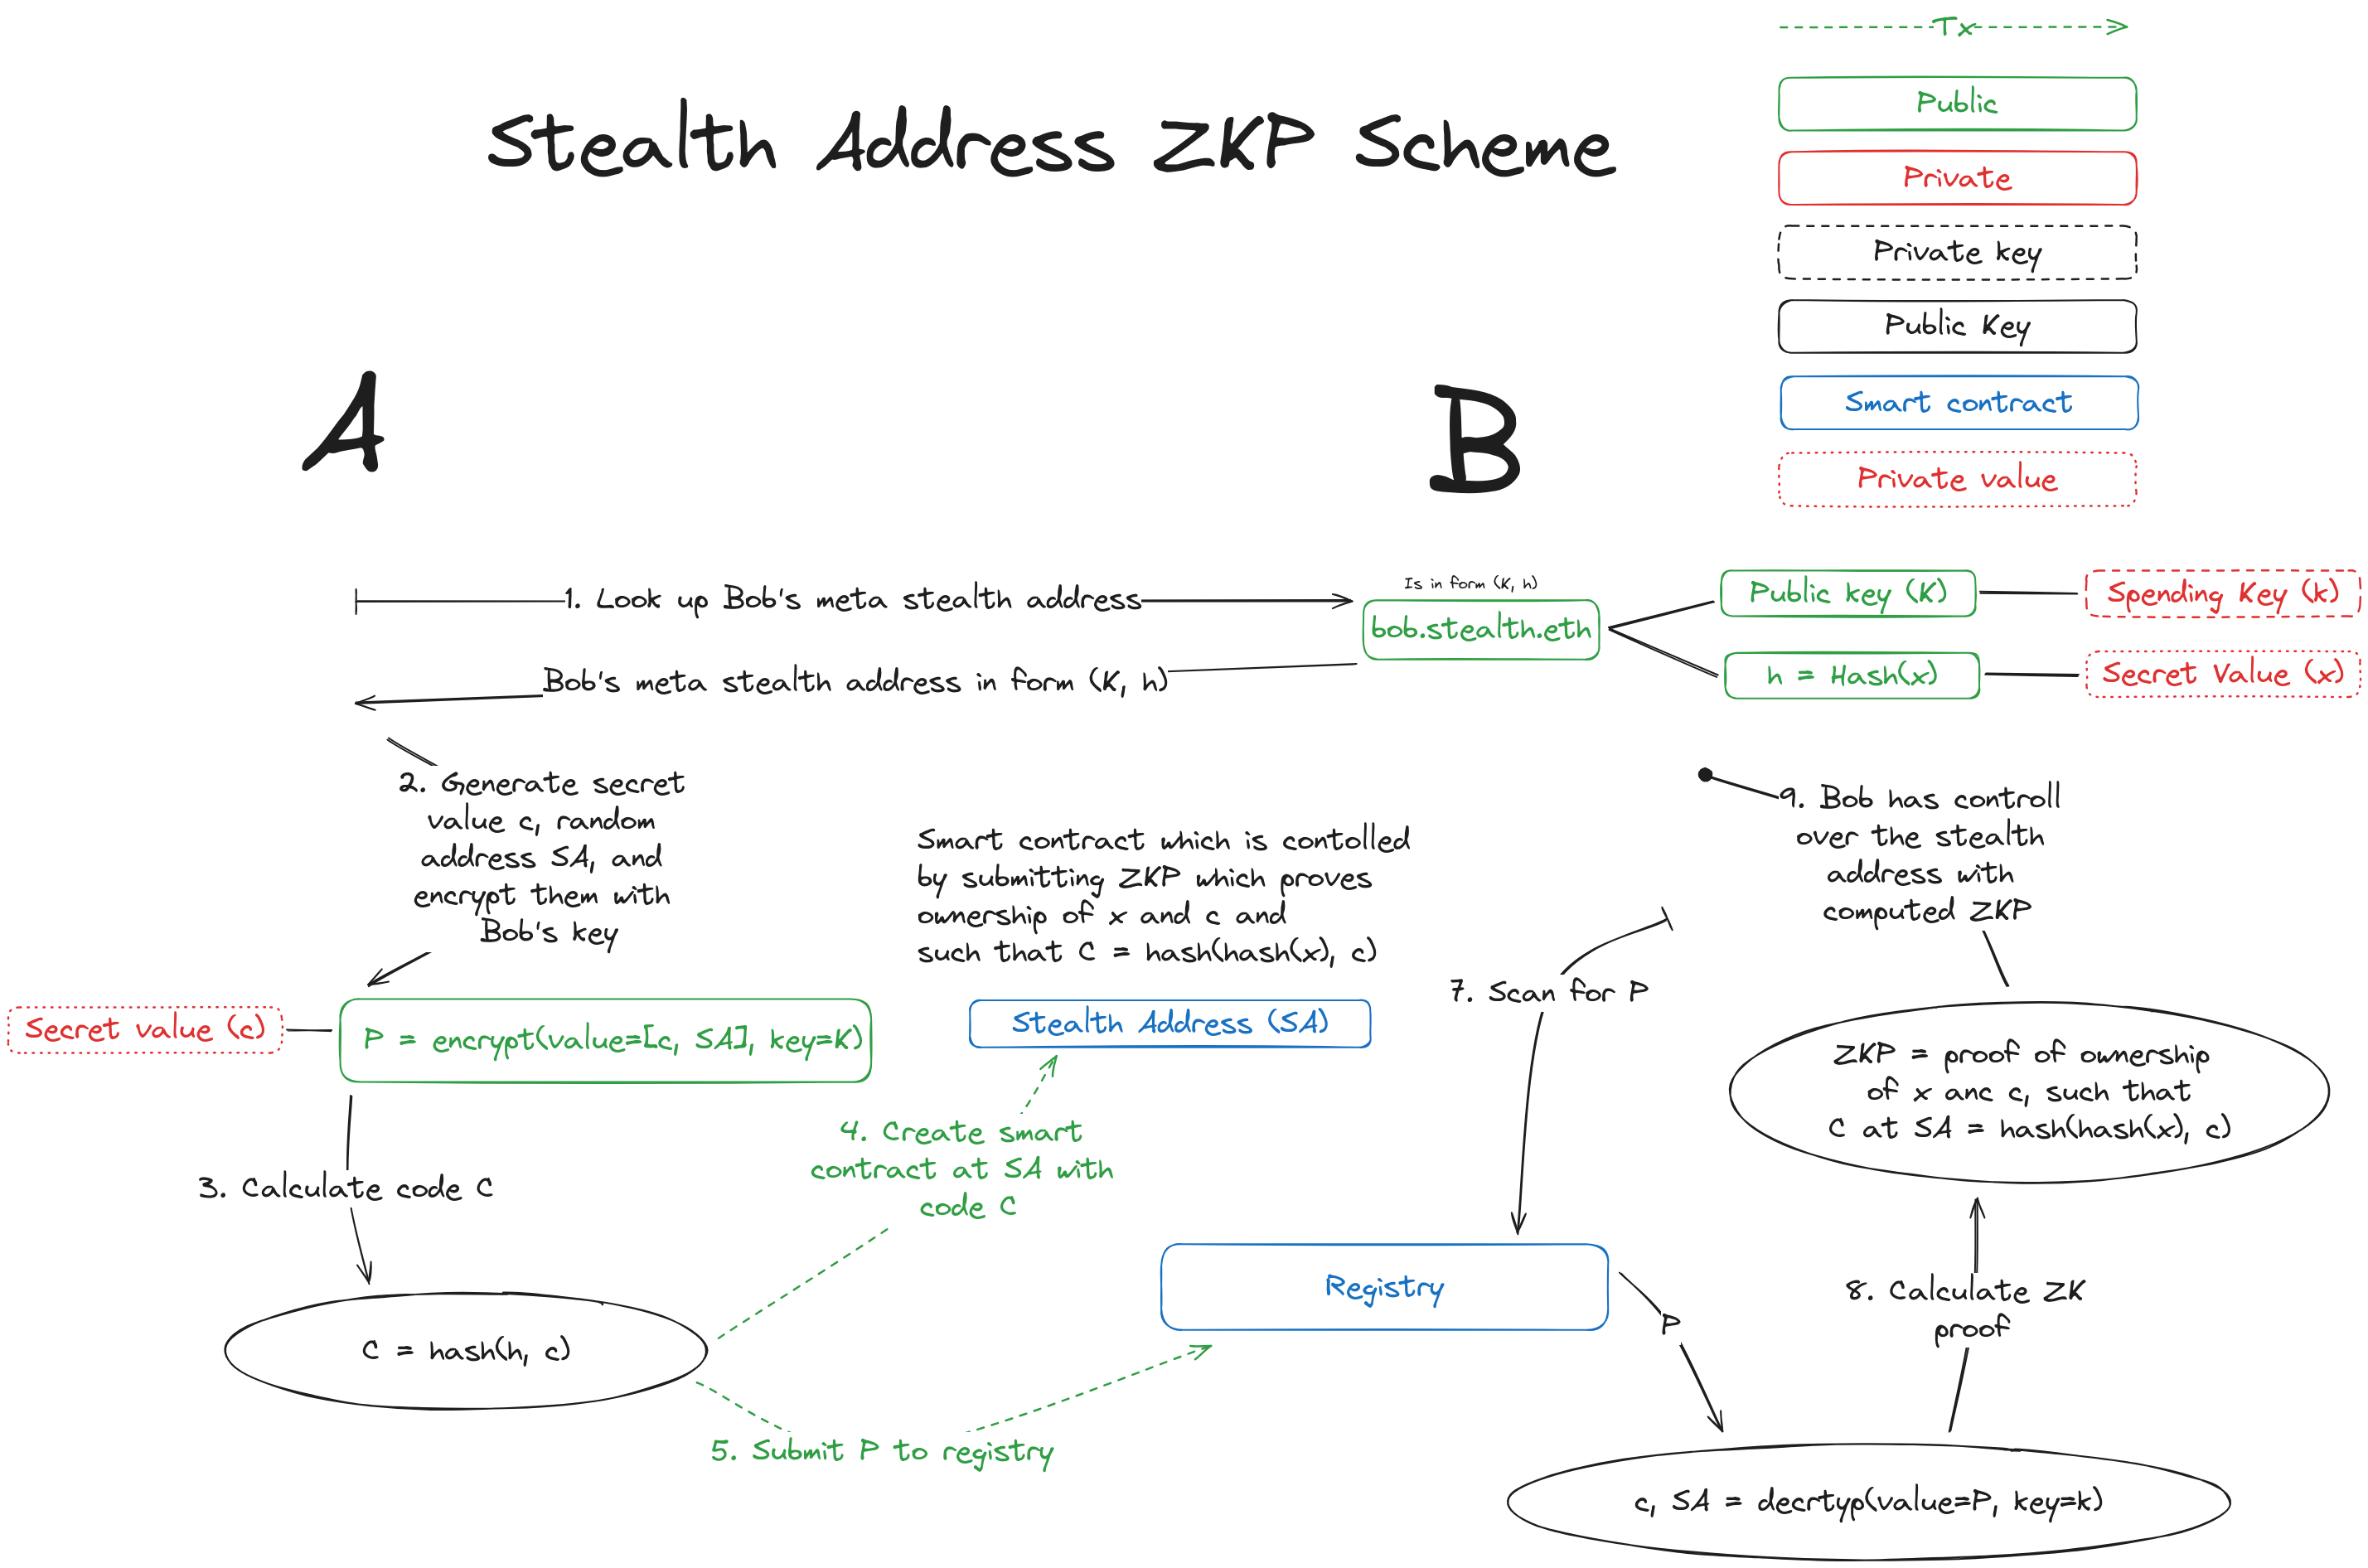
\includegraphics[scale=0.15]{assets/images/solution.png}
    \caption{Solution Design}
    \label{fig:solution}
    \vspace{0.5cm}
\end{figure}

